\section{The lineage \texorpdfstring{$\Pt$}{P\_t}, memory and knowledge \texorpdfstring{$\K$}{K}}
\label{sec:lineage}

\subsection{The commit rule}
\label{sec:commit-rule}

The commit rule is the selection step of the evolutionary search. In avocode it is the only path by
which a version enters $\Pt$ (invariant~1). \avo{commit} runs these checks in order, and the first
that fires decides:
\begin{enumerate}[leftmargin=*,itemsep=1pt]
  \item The working tree must differ from \cmd{HEAD}, ignoring avocode's own files. Otherwise the
    result is a \emph{no-op}: nothing is scored and nothing is recorded.
  \item The scorer runs \emph{now}. There is no way to commit a number that the agent supplies.
  \item A harness error refuses with exit 2.
  \item $\neg\pass$ refuses with exit 1.
  \item The comparator below decides. If it accepts, avocode writes the version.
\end{enumerate}

\paragraph{Notation.} Let $x_t$ be the best version and $x'$ the candidate. Let $\cfgs_t$ and
$\cfgs'$ be their config sets. Let $\sigma \in \{+1, -1\}$ be $+1$ when higher is better. Define
direction-normalized scores $s_c = \sigma f_c(x_t)$ and $s'_c = \sigma' f_c(x')$, so that higher is
always better. Let $\varphi \geq 0$ be the noise floor (\cmd{floor} in \file{.avo/config.json},
default 0). The relative change on config $c$ is
\begin{equation}
  \rho_c =
  \begin{cases}
    0 & \text{if } s'_c = s_c,\\[2pt]
    \dfrac{s'_c - s_c}{|s_c|} & \text{if } s_c \neq 0,\\[6pt]
    \operatorname{sign}(s'_c - s_c)\cdot\infty & \text{if } s_c = 0,\ s'_c \neq s_c.
  \end{cases}
  \label{eq:rho}
\end{equation}

\begin{definition}[Commit rule, default \cmd{reduce = "dominate"}]
\label{def:commit}
A candidate $x'$ becomes $x_{t+1}$ if and only if the tree changed, the scorer ran without a harness
error, $\pass(x')$ holds, and either $\Pt = \emptyset$ or all of the following hold:
\begin{align}
  & \sigma' = \sigma
    && \text{(the direction is frozen)} \label{eq:dir}\\
  & \cfgs_t \subseteq \cfgs'
    && \text{(no measuring less)} \label{eq:cfg}\\
  & \forall c \in \cfgs_t:\ \rho_c \geq -\varphi
    && \text{(no config regresses beyond the band)} \label{eq:noreg}\\
  & \exists c \in \cfgs_t:\ \rho_c > \varphi
    && \text{(some config improves beyond the band)} \label{eq:gain}
\end{align}
\end{definition}

With $\varphi = 0$, conditions \eqref{eq:noreg}--\eqref{eq:gain} reduce to
$\forall c\colon s'_c \geq s_c$ and $\exists c\colon s'_c > s_c$. That is, $x'$ must Pareto-dominate
$x_t$ on the incumbent's configs. The project docs call the rule \emph{dominate-or-tie}, where
``tie'' refers to single configs. A tie on the \emph{whole} vector is refused: ``the lineage records
progress, not equal-scoring rewrites''. \Cref{fig:commit-rule} shows four cases.

\begin{figure}[t]
\centering
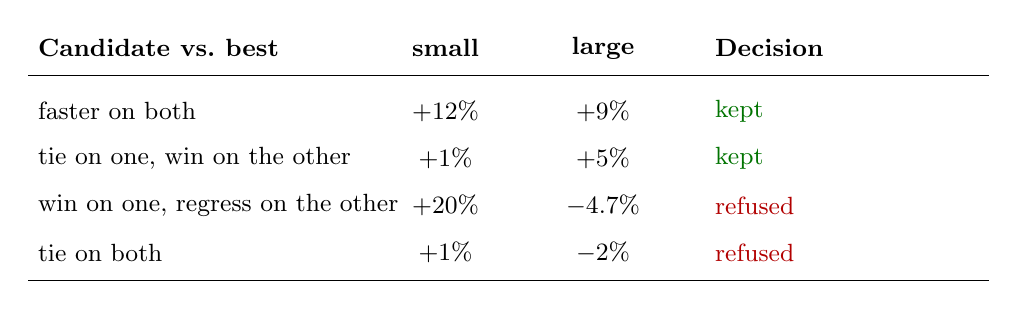
\begin{tikzpicture}[x=1cm,y=1cm]
  \def\row#1#2#3#4#5{%
    \node[anchor=west, font=\small] at (0,#1) {#2};
    \node[font=\small] at (5.3,#1) {#3};
    \node[font=\small] at (7.3,#1) {#4};
    \node[anchor=west, font=\small] at (8.6,#1) {#5};}
  \node[anchor=west, font=\small\bfseries] at (0,0.8) {Candidate vs.\ best};
  \node[font=\small\bfseries] at (5.3,0.8) {\cmd{small}};
  \node[font=\small\bfseries] at (7.3,0.8) {\cmd{large}};
  \node[anchor=west, font=\small\bfseries] at (8.6,0.8) {Decision};
  \draw (0,0.45) -- (12.2,0.45);
  \row{0}{faster on both}{$+12\%$}{$+9\%$}{\textcolor{green!45!black}{kept}}
  \row{-0.6}{tie on one, win on the other}{$+1\%$}{$+5\%$}{\textcolor{green!45!black}{kept}}
  \row{-1.2}{win on one, regress on the other}{$+20\%$}{$-4.7\%$}{\textcolor{red!70!black}{refused}}
  \row{-1.8}{tie on both}{$+1\%$}{$-2\%$}{\textcolor{red!70!black}{refused}}
  \draw (0,-2.15) -- (12.2,-2.15);
\end{tikzpicture}
\caption{The commit rule with a noise floor $\varphi = 3\%$ (the \cmd{fuzzysearch} setting).
Positive values are improvements after direction normalization. A change inside $\pm\varphi$ is a
tie. A win on one config cannot pay for a loss on another, and a tie on every config is not
progress. The third row matches the one real refusal in \cref{sec:eval}.}
\label{fig:commit-rule}
\end{figure}

\paragraph{The opt-in mean rule.} With \cmd{reduce = "mean"}, weights $w_c \geq 0$ (default 1) and
$W = \sum_{c \in \cfgs_t} w_c$, let $M(s) = W^{-1}\sum_{c\in\cfgs_t} w_c s_c$. The candidate is
accepted if the preconditions \eqref{eq:dir}--\eqref{eq:cfg} hold, $W > 0$, and the relative change
of $M$ exceeds $\varphi$. Per-config verdicts are still stored, so a regression that the mean accepts
stays visible. Dominance is the default because ``a mean lets a large win on one config pay for a
regression on another''.

\paragraph{Noise.} $\varphi$ is a \emph{relative} band applied in both directions. Noise inside the
band can neither commit nor block. A regression outside the band still blocks a gain inside it.
avocode has no repeated sampling or confidence interval in the rule; $\varphi$ is the only noise
mechanism, and it should come from measured spread. For \cmd{fuzzysearch}, the scripted reference
steps showed 0--2.5\% interquartile spread, which set $\varphi = 0.03$.

\subsection{Properties of the rule}

\begin{proposition}[Monotone lineage]
\label{prop:monotone}
With $\varphi = 0$ and \cmd{reduce = "dominate"}, for every config $c$ and every pair of versions
$i < j$ that both measure $c$, $s_c(x_j) \geq s_c(x_i)$ (as recorded at commit time).
\end{proposition}
\begin{proof}
By \eqref{eq:cfg}, a config measured by $x_i$ is measured by every later version. By
\eqref{eq:noreg} with $\varphi = 0$, each step does not decrease $s_c$. Induction on $j - i$.
\end{proof}

Three consequences follow, and the implementation relies on each.
\begin{itemize}[leftmargin=*,itemsep=1pt]
  \item \textbf{Best $=$ newest.} \avo{best} returns the version with the highest number, with no
    ranking pass. This is correct only because of \cref{prop:monotone}.
  \item \textbf{Configs only grow.} $\cfgs_t \subseteq \cfgs_{t+1}$. A new config enters with no
    baseline and is binding for every later version. A scorer edit that drops a slow config is
    refused as \cmd{missing-configs}.
  \item \textbf{The direction is frozen.} A flip is refused with the advice to ``start a fresh
    lineage rather than reinterpreting the old scores''.
\end{itemize}
With $\varphi > 0$ the guarantee weakens to $s'_c \geq s_c - \varphi|s_c|$ per step, so a chain of
small in-band losses can drift down on one config over many versions. With the mean rule, only $M$
is monotone. avocode does not re-check these properties; they hold by construction.

\paragraph{Departure from the paper.} The paper keeps a version that ``matches or improves''.
avocode requires a strict gain on at least one config. It also never re-measures the incumbent: the
best version's vector comes from its stored trailer, while the candidate is measured on today's
machine. \Cref{sec:discussion} discusses both choices.

\subsection{Guarding \texorpdfstring{$\f$}{f} against gaming}
\label{sec:gaming}

An optimizer that can edit its own objective will. \Cref{tab:gaming} lists the threats that
avocode considers and how each one is handled. Some are enforced by code. Others rest on
convention: rules in \file{AGENTS.md} and the skills. The gap matters. \avo{commit} stages with
\cmd{git add -A}, so an edit to \file{.avo/score} is committed with the candidate. A scorer edit that
drops a config or flips the direction is caught. A scorer edit that simply inflates its numbers is
not caught by the harness. The benchmarks close part of this gap with a hash gate over protected
files inside the scorer and an external audit after the run (\cref{sec:eval-bench}).

\begin{table}[t]
\centering\small
\caption{Threats to the integrity of $\f$ and how avocode handles them.}
\label{tab:gaming}
\begin{tabularx}{\linewidth}{@{}X X l@{}}
\toprule
Threat & Mechanism & Kind \\
\midrule
Commit a number that was not measured & \avo{commit} always re-scores & enforced \\
Fast but wrong candidate & $\pass$ gate before any ranking & enforced \\
A win on one config pays for a loss & dominance is the default & enforced \\
Improve by dropping a slow config & \eqref{eq:cfg}: \cmd{missing-configs} & enforced \\
Flip the metric direction & \eqref{eq:dir}: \cmd{direction-changed} & enforced \\
Noise commits a non-change & floor $\varphi$ & enforced, opt-in \\
A typo in the config disables the gate & malformed config $\Rightarrow$ all defaults & enforced \\
Hand-written version commit & only trailer-bearing commits count & convention \\
Edit \file{.avo/score} to pass & rules in \file{AGENTS.md} and skills; bench hash gate & convention / bench \\
Edit \file{lineage/} & rules; the comparator never reads \file{lineage/} & convention + design \\
\bottomrule
\end{tabularx}
\end{table}

\subsection{Persisting a version}

A version exists if and only if a commit reachable from \cmd{HEAD} carries a valid
\cmd{Avo-Version} trailer and a valid \cmd{Avo-Score} trailer. Nothing else defines a version. The
commit message has three paragraphs:
\begin{lstlisting}
avo v3: 0.408 ms

partition (pigeonhole) hash index: cut each word into k+1 segments ...

Avo-Version: 3
Avo-Score: {"primary":0.408,"unit":"ms","higher_is_better":false,
            "scores":{"small":0.309,"large":0.507}}
\end{lstlisting}
Each version has three records with different jobs (\cref{fig:records}).
\begin{enumerate}[leftmargin=*,itemsep=1pt]
  \item \textbf{The commit and its trailers}: exactly what the comparator reads back, and nothing
    more. A damaged note or a deleted Markdown file cannot change a decision.
  \item \textbf{A git note} under \cmd{refs/notes/avo}: the full attempt, logs and per-config deltas.
  \item \textbf{\file{lineage/vNNN.md}}: a readable page with the score table, parent, rationale and
    diffstat. This page is also part of $\K$ (\cref{sec:knowledge}).
\end{enumerate}
The lineage is read with one \cmd{git log} using ASCII unit and record separators. Rules for
robustness: the last trailer wins (a rebase can prepend an old body), malformed trailers are skipped
with a warning, and for duplicate numbers the newest commit wins. Because the lineage is read from
the ancestry of \cmd{HEAD}, each branch carries its own lineage.

\begin{figure}[t]
\centering
\begin{tikzpicture}[node distance=0.35cm]
  \node[store, text width=5.6cm] (c) {\textbf{commit} \texttt{3d1e5ce}\\
    \texttt{avo v3: 0.408 ms}\\ \texttt{Avo-Version: 3}\\ \texttt{Avo-Score: \{...\}}};
  \node[store, text width=5.6cm, below=of c] (n) {\textbf{git note} \texttt{refs/notes/avo}\\
    full attempt, logs, per-config deltas};
  \node[store, text width=5.6cm, below=of n] (l) {\textbf{\file{lineage/v003.md}}\\
    score table, parent v2, \emph{why}, diffstat};
  \node[store, text width=5.6cm, below=of l] (m) {\textbf{memory} \texttt{avo-v3}\\
    parent link \texttt{avo-v2}, rationale};
  \node[draw, dashed, rounded corners, fit=(c)(n)(l)(m), inner sep=6pt,
        label={[font=\small\bfseries]above:lineage (committed)}] (L) {};
  \node[store, fill=gray!8, text width=4.6cm, right=1.6cm of n] (a) {\file{.avo/attempts.jsonl}\\
    every scorer run, pass or fail};
  \node[store, fill=gray!8, text width=4.6cm, below=of a] (w) {\file{.avo/worktrees/}\\ fan-out probes};
  \node[store, fill=gray!8, text width=4.6cm, below=of w] (r) {\file{.avo/runs/}\\ run manifests, agent logs};
  \node[draw, dashed, rounded corners, fit=(a)(w)(r), inner sep=6pt,
        label={[font=\small\bfseries]above:trajectory (gitignored)}] (T) {};
\end{tikzpicture}
\caption{Lineage versus trajectory, for version v3 of the \cmd{fuzzysearch} run. The lineage
records accepted versions. The trajectory records how they were reached. Memory is committed in
the JSONL fallback and lives in the beads database otherwise.}
\label{fig:records}
\end{figure}

\paragraph{Lineage versus trajectory.} avocode keeps \emph{what survived} apart from \emph{how it was
reached}. Trajectory paths are gitignored and also unstaged after \cmd{git add -A}, in case a repo
already tracked them. avocode's own files are also excluded from the dirty check. Without this, the
memory record written after v1 would make the next turn see a change the agent never made, score it,
refuse it, record the refusal, and dirty the tree again. The project calls this class of bug
\emph{self-perturbation}; it appeared in three separate development slices.

\subsection{What happens on refusal}
\label{sec:refusal}

A refused candidate leaves no trace in git. It is recorded in three other places.
\begin{enumerate}[leftmargin=*,itemsep=1pt]
  \item \textbf{Trajectory}: the attempt is already in \file{.avo/attempts.jsonl}.
  \item \textbf{Memory}: a dead-end record keyed by content,
    $\mathit{key} = \mathrm{sha256}(\mathit{reason} \,\|\, \mathit{vector})_{[0:8]}$, so a repeat of
    the same dead end updates one record instead of adding a new one.
  \item \textbf{Output}: the reason names the configs and deltas, for example \emph{``\,`small'
    regressed (worst: small $-4.74\%$) (floor $\pm 3.00\%$)''}.
\end{enumerate}
Harness errors are \emph{not} recorded as dead ends, because ``a harness error taught us nothing
about the candidate''. The refused candidate stays in the working tree, so the agent can keep
working on it. The skill tells the agent to add an insight with \avo{mem add} when it knows
\emph{why} a change failed, because ``an unrecorded refusal is one the next session earns again''.

\subsection{Memory}

The paper's agent remembers through its conversation history. avocode moves memory out of the agent
and into the repository, which is what makes the operator restartable and agent-agnostic. A memory
record has the shape \cmd{\{ts, kind, key, text, version, parent\}}, with four kinds:
\cmd{insight}, \cmd{version}, \cmd{failure} and \cmd{intervention}. If the beads issue tracker
\citep{yegge2025beads} is present, records become beads, and version records are linked parent to
child, which mirrors the lineage as a dependency graph. Otherwise they go to
\file{lineage/memory.jsonl}, append-only with last-write-wins per key. The agent reads the same JSON
in both cases. \avo{mem prime} prints insights, ``dead ends (do not re-try these)'' and committed
versions. Interventions are left out on purpose, so old directives do not echo into new sessions.

\subsection{Knowledge \texorpdfstring{$\K$}{K}}
\label{sec:knowledge}

$\K$ has two Markdown collections: \file{knowledge/} (``what we were told'': docs and papers) and
\file{lineage/} (``what we learned''). Both are indexed by qmd \citep{lutke2025qmd}, which combines BM25,
vector search, LLM query expansion and a local reranker. Because \avo{commit} already writes
\file{lineage/vNNN.md}, the question ``what did I already try about register pressure?'' is the same
query as ``what do the docs say about it?''. This turns the paper's observation that the agent
``frequently examines multiple prior implementations in $\Pt$'' into a single search over both.

Without a project-local qmd index, a local scan returns the same JSON shape. Its score is the
fraction of distinct query terms that match, and it says it is not BM25. Documents can be added from
the web with \avo{know search --ingest} or \avo{know add}. Each added file records its
\cmd{source}, \cmd{title}, \cmd{fetched-at} time and \cmd{via} backend in front matter, so a
claim in $\K$ can be traced and checked later. Re-adding a page with the same body is a no-op; a
different body is refused without \cmd{--force}.
